%!TEX TS-program = xelatex
\documentclass[notes,12pt, aspectratio=169]{beamer}

\usepackage{amsmath,amsfonts,amssymb,amsthm,mathtools}  % пакеты для математики
%\usepackage{minted}

\usepackage[english, russian]{babel} % выбор языка для документа
\usepackage[utf8]{inputenc} % задание utf8 кодировки исходного tex файла
\usepackage[X2,T2A]{fontenc}        % кодировка

\usepackage{fontspec}         % пакет для подгрузки шрифтов
\setmainfont{Helvetica}  % задаёт основной шрифт документа

% why do we need \newfontfamily:
% http://tex.stackexchange.com/questions/91507/
\newfontfamily{\cyrillicfonttt}{Helvetica}
\newfontfamily{\cyrillicfont}{Helvetica}
\newfontfamily{\cyrillicfontsf}{Helvetica}

\usepackage{unicode-math}     % пакет для установки математического шрифта
% \setmathfont{Neo Euler} % шрифт для математики

\usepackage{polyglossia}      % Пакет, который позволяет подгружать русские буквы
\setdefaultlanguage{russian}  % Основной язык документа
\setotherlanguage{english}    % Второстепенный язык документа

% Шрифт для кода
\setmonofont[Scale=0.85]{Monaco}
\usepackage{verbments}

\usepackage{pgfpages}
% These slides also contain speaker notes. You can print just the slides,
% just the notes, or both, depending on the setting below. Comment out the want
% you want.
%\setbeameroption{hide notes} % Only slide
%\setbeameroption{show only notes} % Only notes
%\setbeameroption{show notes on second screen=right} % Both

\usepackage{array}

\usepackage{tikz}
\usepackage{verbatim}
\setbeamertemplate{note page}{\pagecolor{yellow!5}\insertnote}
\usetikzlibrary{positioning}
\usetikzlibrary{snakes}
\usetikzlibrary{calc}
\usetikzlibrary{arrows}
\usetikzlibrary{decorations.markings}
\usetikzlibrary{shapes.misc}
\usetikzlibrary{matrix,shapes,arrows,fit,tikzmark}

\usepackage{hyperref}
\usepackage{lipsum}
\usepackage{multimedia}
\usepackage{multirow}
\usepackage{dcolumn}
\usepackage{bbm}
\newcolumntype{d}[0]{D{.}{.}{5}}

\usepackage{changepage}
\usepackage{appendixnumberbeamer}
\newcommand{\beginbackup}{
   \newcounter{framenumbervorappendix}
   \setcounter{framenumbervorappendix}{\value{framenumber}}
   \setbeamertemplate{footline}
   {
     \leavevmode%
     \hline
     box{%
       \begin{beamercolorbox}[wd=\paperwidth,ht=2.25ex,dp=1ex,right]{footlinecolor}%
%         \insertframenumber  \hspace*{2ex} 
       \end{beamercolorbox}}%
     \vskip0pt%
   }
 }
\newcommand{\backupend}{
   \addtocounter{framenumbervorappendix}{-\value{framenumber}}
   \addtocounter{framenumber}{\value{framenumbervorappendix}} 
}

% для имитации питоновского синтаксиса 
\newcommand{\pgr}[1]{{\color{green} \textbf{#1}}}


%%%%%%%%%% Работа с картинками %%%%%%%%%
\usepackage{graphicx}                  % Для вставки рисунков
\usepackage{graphics}
\graphicspath{{images/}}    % можно указать папки с картинками
\usepackage{wrapfig}                   % Обтекание рисунков и таблиц текстом

\usepackage[space]{grffile}
\usepackage{booktabs}

% These are my colors -- there are many like them, but these ones are mine.
\definecolor{blue}{RGB}{0,114,178}
\definecolor{red}{RGB}{213,94,0}
\definecolor{yellow}{RGB}{240,228,66}
\definecolor{green}{RGB}{0,128, 0}

\hypersetup{
  colorlinks=true,
  linkbordercolor = {white},
  urlcolor=blue
}


%% I use a beige off white for my background
\definecolor{MyBackground}{RGB}{255,253,218}

%% Uncomment this if you want to change the background color to something else
%\setbeamercolor{background canvas}{bg=MyBackground}

%% Change the bg color to adjust your transition slide background color!
\newenvironment{transitionframe}{
  \setbeamercolor{background canvas}{bg=yellow}
  \begin{frame}}{
    \end{frame}
}

\setbeamercolor{frametitle}{fg=blue}
\setbeamercolor{title}{fg=black}
\setbeamertemplate{footline}[frame number]
\setbeamertemplate{navigation symbols}{} 
\setbeamertemplate{itemize items}{-}
\setbeamercolor{itemize item}{fg=blue}
\setbeamercolor{itemize subitem}{fg=blue}
\setbeamercolor{enumerate item}{fg=blue}
\setbeamercolor{enumerate subitem}{fg=blue}
\setbeamercolor{button}{bg=MyBackground,fg=blue,}


% If you like road maps, rather than having clutter at the top, have a roadmap show up at the end of each section 
% (and after your introduction)
% Uncomment this is if you want the roadmap!
% \AtBeginSection[]
% {
%    \begin{frame}
%        \frametitle{Roadmap of Talk}
%        \tableofcontents[currentsection]
%    \end{frame}
% }
\setbeamercolor{section in toc}{fg=blue}
\setbeamercolor{subsection in toc}{fg=red}
\setbeamersize{text margin left=1em,text margin right=1em} 

% списки, которые растягиваются на всю величину слайда 
\newenvironment{wideitemize}{\itemize\addtolength{\itemsep}{10pt}}{\enditemize}

\usepackage{xcolor}

% Syntax: \colorboxed[<color model>]{<color specification>}{<math formula>}
\newcommand*{\colorboxed}{}
\def\colorboxed#1#{%
	\colorboxedAux{#1}%
}

\newcommand*{\colorboxedAux}[3]{%
	% #1: optional argument for color model
	% #2: color specification
	% #3: formula
	\begingroup
	\colorlet{cb@saved}{.}%
	\color#1{#2}%
	\boxed{%
		\color{cb@saved}%
		#3%
	}%
	\endgroup
}

\usepackage{pgfplots}
\usepackage{tikz}

\DeclareMathOperator{\logloss}{logloss}
\DeclareMathOperator{\Softmax}{Softmax}

\title[]{\textcolor{blue}{Машинное обучение 2: Судный день}}
\author{Ульянкин Филипп}
\date{\today}

\usepackage{ulem}
\usepackage{MnSymbol,wasysym}

\begin{document}

%%% TIKZ STUFF
\tikzset{   
        every picture/.style={remember picture,baseline},
        every node/.style={anchor=base,align=center,outer sep=1.5pt},
        every path/.style={thick},
        }
\newcommand\marktopleft[1]{%
    \tikz[overlay,remember picture] 
        \node (marker-#1-a) at (-.3em,.3em) {};%
}
\newcommand\markbottomright[2]{%
    \tikz[overlay,remember picture] 
        \node (marker-#1-b) at (0em,0em) {};%
}
\tikzstyle{every picture}+=[remember picture] 
\tikzstyle{mybox} =[draw=black, very thick, rectangle, inner sep=10pt, inner ysep=20pt]
\tikzstyle{fancytitle} =[draw=black,fill=red, text=white]
%%%% END TIKZ STUFF

% Title Slide

\begingroup
\setbeamercolor{background canvas}{bg = black}
\begin{frame}[plain]
\begin{center}
	\Huge{\color{red}{ВНИМАНИЕ!}}
\end{center}

\begin{center}
	\color{white}{ДАННЫЙ КУРС СОДЕРЖИТ БОЛЬШОЕ КОЛИЧЕСТВО РАЗНООБРАЗНОГО КОДА И ЗАДАНИЙ ДЛЯ САМОСТОЯТЕЛЬНОГО РЕШЕНИЯ. \\
		\vspace{3mm}
		НА ПЕРВЫЙ ВЗГЛЯД ОН МОЖЕТ ПОКАЗАТЬСЯ СЛОЖНЫМ И ТРАВМИРОВАТЬ НЕПОДГОТОВЛЕННУЮ ПСИХИКУ. ТАКЖЕ ОН СОДЕРЖИТ БОЛЬШОЕ КОЛИЧЕСТВО НЕУДАЧНЫХ ШУТОК И НЕУМЕСТНЫХ ОТСЫЛОК. \\ 
		\vspace{3mm}
		В СВЯЗИ С ЭТИМ КУРС НЕ РЕКОМЕНДУЕТСЯ ПРОСЛУШИВАТЬ \ldots{ } НИКОМУ.}
\end{center}
\end{frame}
\endgroup


\begin{frame}
\maketitle
\centering \textbf{\color{blue} Посиделка 1:}  вводная с кучей повторения
\end{frame}


\begin{frame}{Agenda}
\begin{wideitemize}
	\item  Бюрократия
	\item  Какие задачи решают в машинном обучении  и чем мы займёмся
	\item  Откуда берутся функции потерь и какими они бывают 
	\item  Что такое регуляризация 
	\item  Что такое BVD
\end{wideitemize} 
\end{frame}


\begin{transitionframe}
	\begin{center}
	%\centering \includegraphics[scale = 0.03]{pac-man.png}
		\Huge Правила игры
	\end{center}
\end{transitionframe}


\begin{frame}{Про пары}
	\begin{wideitemize}
		\item  что-то неясно $\Rightarrow$ \alert{ ПЕРЕБЕЙ И СПРОСИ}
		
		\item  презентаций будет мало, заводите тетрадки :3 
		
		\item все материалы можно найти на  \href{https://github.com/FUlyankin/ml_ranepa}{страничке курса}
	\end{wideitemize} 
\end{frame}


\begin{frame}{Что почитать}
	\begin{wideitemize}
		\item  \href{https://ml-handbook.ru/}{Онлайн-учебник по машинному обучению от ШАД}
		
		\item  \href{https://github.com/esokolov/ml-course-hse}{Конспекты Жени Соколова}
	\end{wideitemize} 
\end{frame} 


\begin{transitionframe}
	\begin{center}
			\Huge Карта ML
		\end{center}
% \centering \href{https://vk.com/skialz}{\includegraphics[scale = 0.25]{story.png}}
\end{transitionframe}


\begin{frame}[plain]
\begin{center}
	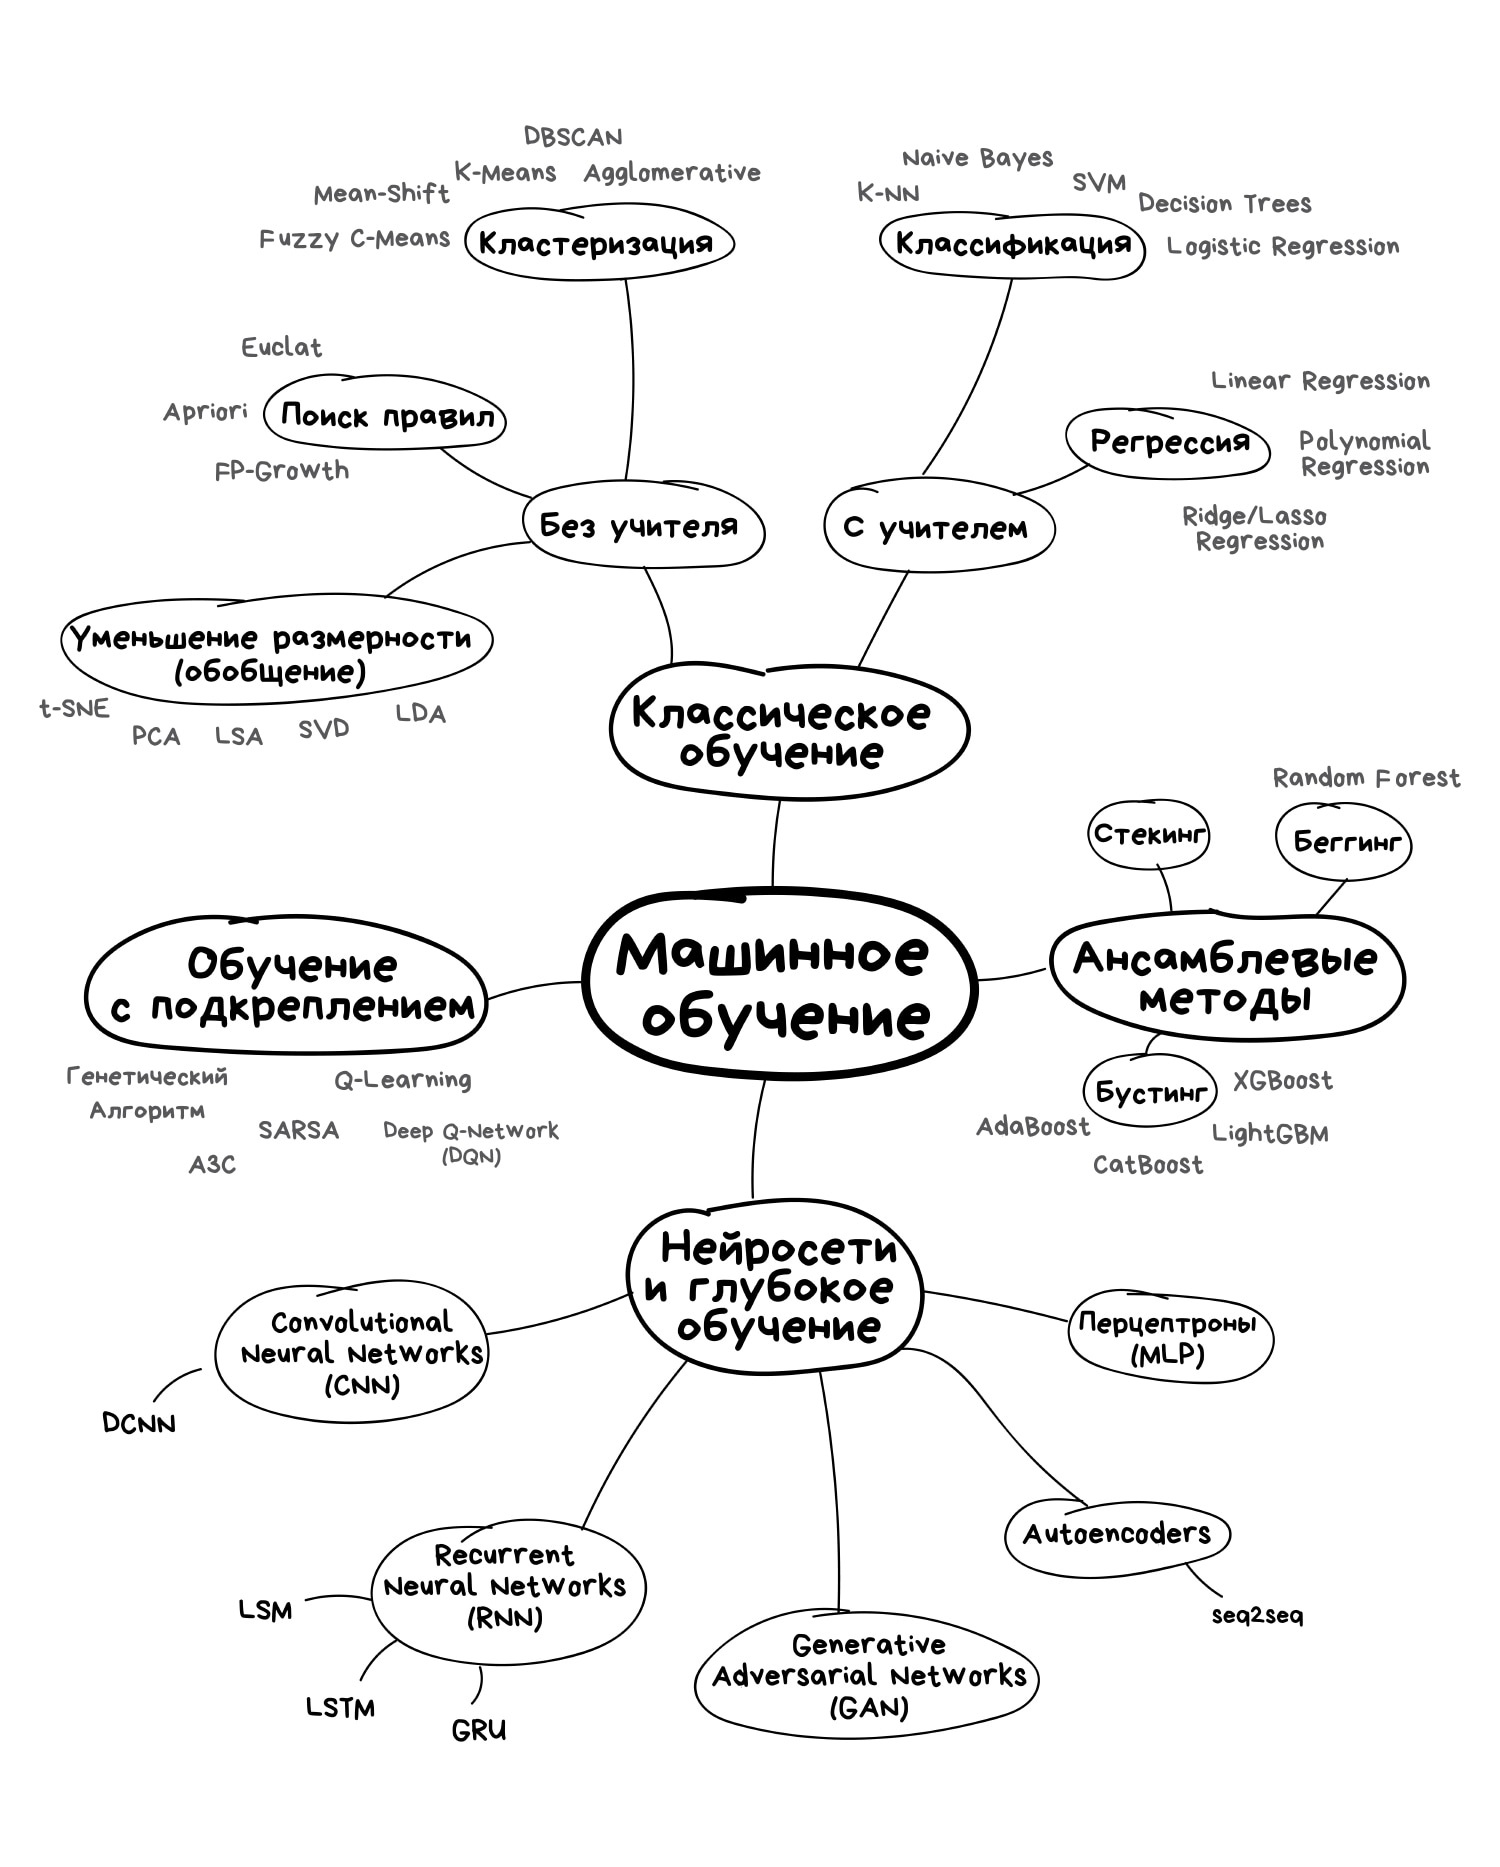
\includegraphics[width=.45\linewidth]{ds.jpeg}
\end{center}
\end{frame} 


\begin{frame}[plain]
	\begin{center}
		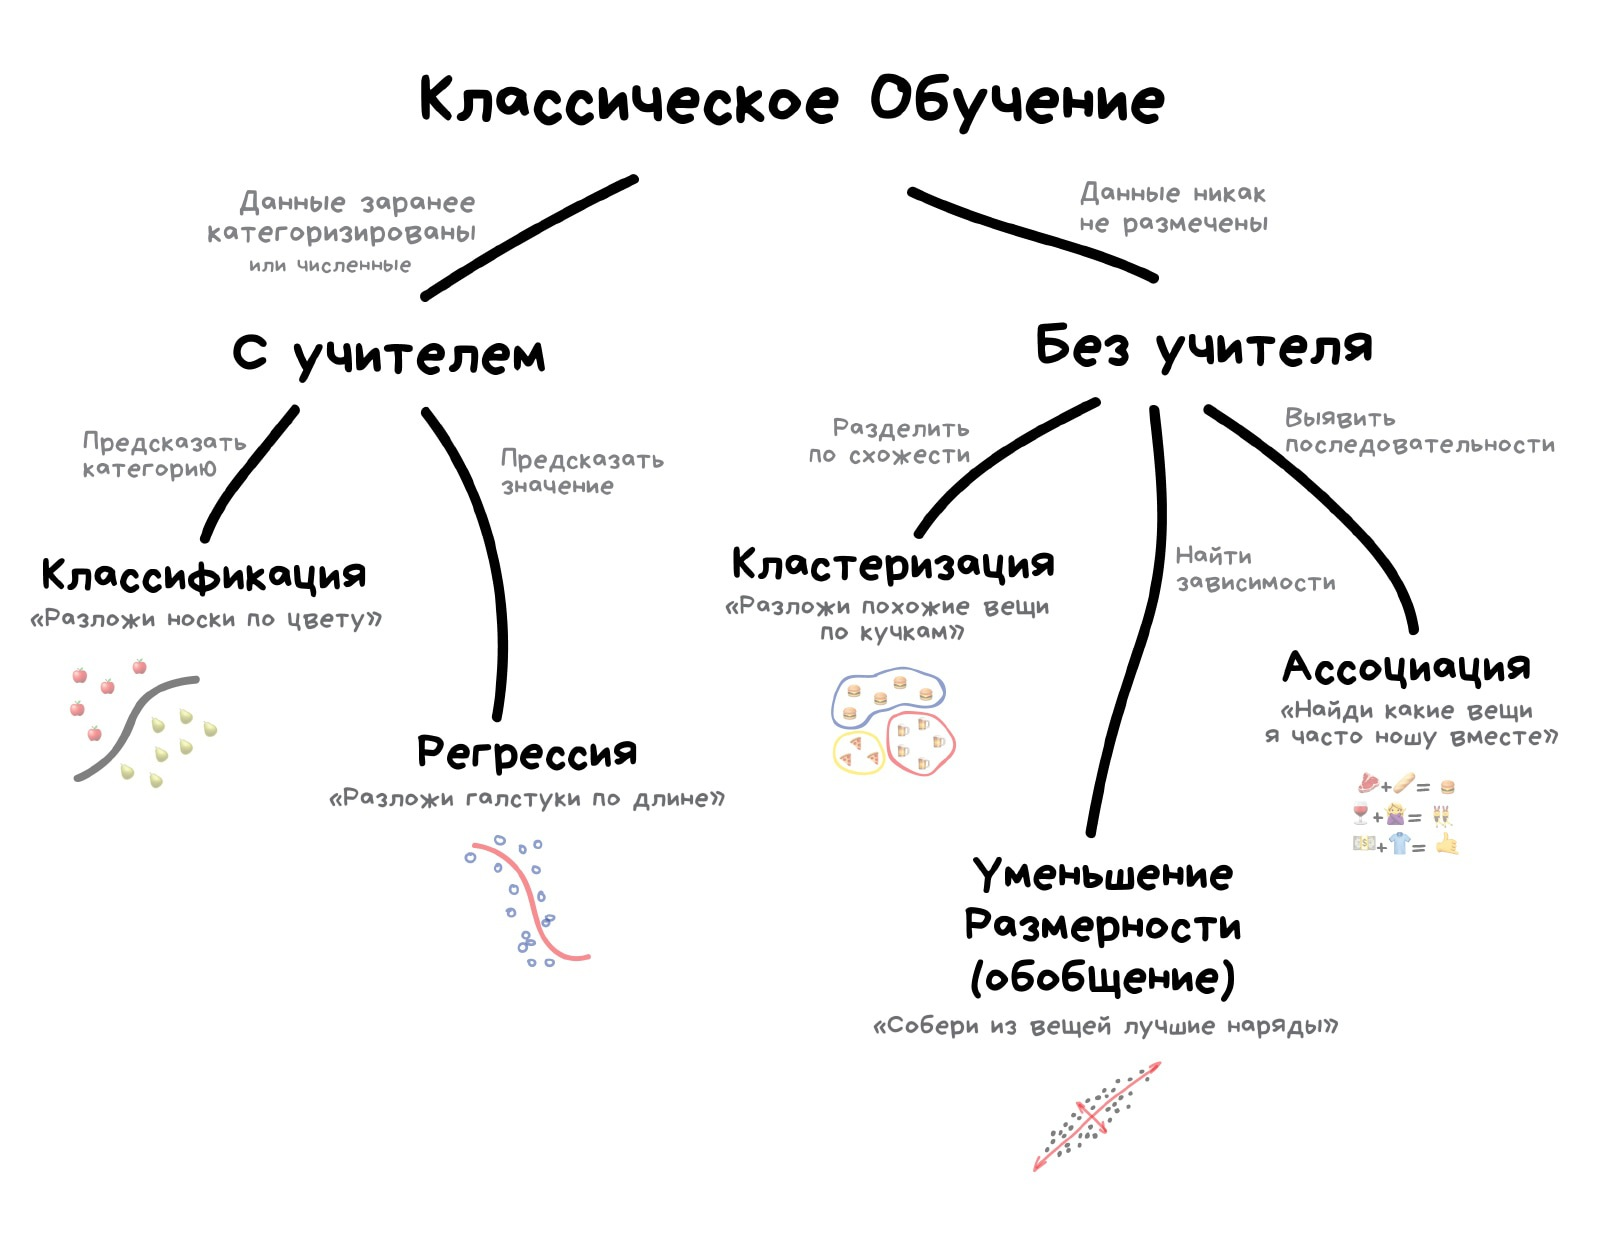
\includegraphics[width=.7\linewidth]{ml.jpeg}
	\end{center}
\end{frame} 


\begin{transitionframe}
	\begin{center}
		\Huge Обучение с учителем: регрессия 
	\end{center}
	% \centering \href{https://vk.com/skialz}{\includegraphics[scale = 0.25]{story.png}}
\end{transitionframe}


\begin{frame}{Базовая постановка}
	
	\begin{wideitemize}
		
		\item $(x_i, y_i)_{i=1}^n$ — обучающая выборка
		
		\item $a(x)$ — алгоритм, модель
		
		\item $Q(a, X)$ — функционал ошибки алгоритма $a$ на выборке $X$ 
		
		\item Обучение:  $a(x) = \arg \min_{a \in A} Q(a, X)$
	
	\end{wideitemize}

		\[
		Q(a, X) = \frac{1}{n}  \sum_{i=1}^n  \underbrace{L(y_i, a(x_i)) }_{\text{\textcolor{red}{Функция потерь}}} +  \lambda \cdot \underbrace{R(w)}_{\text{\textcolor{red}{Регуляризатор}}} \to  \min_w 
		\]

\end{frame}


\begin{frame}{Регрессия}
		\[
		Q(a, X) = \frac{1}{n}  \sum_{i=1}^n  \underbrace{L(y_i, a(x_i)) }_{\text{\textcolor{red}{Функция потерь}}} +  \lambda \cdot \underbrace{R(w)}_{\text{\textcolor{red}{Регуляризатор}}} \to  \min_w 
		\]
	
	\begin{wideitemize}
	\item Обучение идёт на действительные числа $y_i \in \mathbb{R}$

	\only<2>{
	\item \alert{Квадратичное отклонение:}
	\[
		L(y, a) = (a - y)^2
	\]}
	
	\only<3>{
	\item \alert{Абсолютное отклонение:}
	\[
	L(y, a) = |a - y|
	\]}

	\only<4>{
	\item \alert{Функция потерь Хубера:}
	\[
	L_\delta(y, a)
	=
	\left\{
	\begin{aligned}
		&\frac12 (y - a)^2, \quad |y - a| < \delta \\
		&\delta \left(
		|y - a| - \frac12 \delta
		\right), \quad |y - a| \geq \delta
	\end{aligned}
	\right.
	\]}
	
	\only<5>{
	\item \alert{Log-Cosh:}
		\[
		L(y, a) = \log \cosh(a - y)
		\]
	}
	\end{wideitemize}
\end{frame}


\begin{frame}{Функции потерь для регрессии}
	\begin{center}
		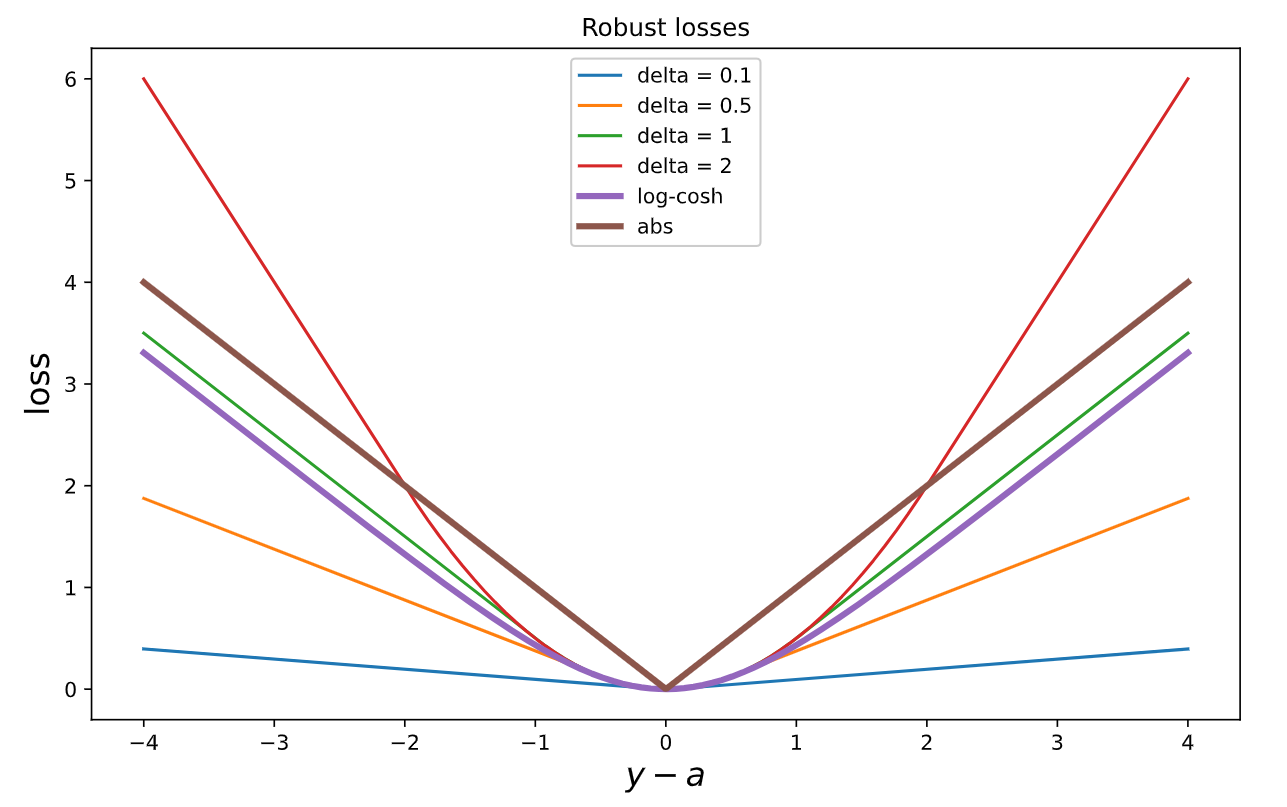
\includegraphics[width=.8\linewidth]{huber.png}
	\end{center}
\end{frame} 


\begin{frame}{Инженерный подход к машинному обучению}
	\begin{wideitemize}
		\item Есть проблема, есть функция потерь которая штрафует за ошибку
		
		\item  Если у этой функции потерь есть какие-то проблемы, стараемся придумать костыли, чтобы их починить 
		
		\item Квадратичные потери чувствительны к выбросам, абсолютные хуже оптимизируются $\Rightarrow$ скрестим их в потери Хубера
		
		\item Вторая производная потерь хубера имеет разрывы $\Rightarrow$  находим похожую гладкую функцию, получаем Log-Cosh
		
		\item Статистические свойства не очень нас интересуют
	\end{wideitemize}
\end{frame} 


\begin{frame}{Ещё примеры: Квантильная  ошибка}
	
	\[
	L(y, a) = k_1 \cdot |y -  a| \cdot  [y < a]    +  k_2 \cdot |y - a| \cdot  [y \ge a]
	\]
	
	\begin{wideitemize}
		
		\item  Сложно минимизировать
		
		\item  В качестве прогноза строится $\tau$-квантиль, где $\tau = \frac{k_2}{k_1 + k_2}$
	\end{wideitemize}
\end{frame}



\begin{frame}{Ещё примеры: MSLE}
	\[
	L(y, a) = (\log(a + 1) - \log(y + 1))^2
	\]
	
	\begin{wideitemize}
		
		\item  Подходит для задач с неотрицательной целевой переменной и неотрицательными прогнозами модели
		
		\item  За счёт логарифмирования ответов и прогнозов мы скорее штрафуем за отклонения
		в порядке величин, чем за отклонения в их значениях
		
		\item Логарифм не является симметричной функцией,
		и поэтому данная функция потерь штрафует заниженные прогнозы сильнее,
		чем завышенные
	\end{wideitemize}

\end{frame}


\begin{frame}{Вероятностный подход к машинному обучению}
	\begin{wideitemize}
		\item  Обучающая выборка и ответы на ней $(x_1, y_1), (x_2, y_2), \ldots, (x_n, y_n)$ приходят к нам из какого-то распределения
		
		\[
		p(x, y) = p(x \mid y) \cdot p(y)
		\]
		
		\pause
		
		\item Параметризуем это распределение с помощью какой-то модели
		
		\[
		p(x, y \mid \theta) \propto p(x \mid y, \theta) \cdot p(y)
		\]
		
		
		\only<3>{
		\item Если предположить, что вектор параметров~$\theta$ константа, получим \alert{метод макимального правдоподобия}
		
		\[
		\hat{\theta}
		=
		\arg \max_\theta
		L(\theta)
		=
		\arg \max_\theta
		\prod_{i = 1}^{n} p(y_i \mid x_i, \theta) =
		\arg \max_\theta
		\prod_{i = 1}^{n} p(x_i \mid d y_i, \theta),
		\]}
	
		\only<4>{
		\item Если предположить, что вектор параметров~$\theta$ случайная величина, мы приоткроем для себя дверь в \alert{Байесовские методы} 
		}
		
	\end{wideitemize}
\end{frame} 


\begin{frame}{Среднеквадратичная ошибка}
	
	\[
	MSE = \frac{1}{n} \sum_{i=1}^n (a(x_i) - y_i)^2
	\]
	
	\begin{wideitemize}
		
		\item  Легко минимизировать
		
		\item  Чувствительна к выбросам 
		
		\item  В качестве прогноза строится $\mathbb{E}(y \mid X)$
		
		\item  Обучение эквивалентно оптимизации правдоподобия для  \[ y_i \mid x_i \sim N(a(x_i), \sigma^2 ) \]
		
		\item На семинарах будем решать такие задачи :) 
		
	\end{wideitemize}
\end{frame}


\begin{frame}{Резюме}
	\begin{wideitemize}
		\item Есть два подхода к придумыванию функций потерь: инженерный и вероятностный
		
		\item Очень часто функции потерь — замаскированное правдоподобие  
		
		\item  Если уметь сопоставлять функцию потерь вероятностной модели, можно лучше понимать зону её применимости
		
		\item  Подходы можно комбинировать
	\end{wideitemize}
\end{frame}


\begin{transitionframe}
	\begin{center}
		\Huge Обучение с учителем: классификация
	\end{center}
	% \centering \href{https://vk.com/skialz}{\includegraphics[scale = 0.25]{story.png}}
\end{transitionframe}


\begin{frame}{Классификация}
		\[
		Q(a, X) = \frac{1}{n}  \sum_{i=1}^n  \underbrace{L(y_i, a(x_i)) }_{\text{\textcolor{red}{Функция потерь}}} +  \lambda \cdot \underbrace{R(w)}_{\text{\textcolor{red}{Регуляризатор}}} \to  \min_w 
		\]
	
	\begin{wideitemize}
		\item Обучение идёт на класс $y_i \in \{-1, 1\}$
		
		\only<2>{
			\item \alert{Доля неправильных ответов:}
			\[
			Q(a, X) = \sum_{i=1}^n [a(x_i) \ne y_i]
			\]}
		
		\only<3>{
			\item \alert{Доля неправильных ответов:}
			\[
			Q(a, X) = \sum_{i=1}^n [a(x_i) \ne y_i] = \sum_{i=1}^n [\underbrace{y_i  \cdot  \langle w, x_i \rangle}_{\text{\textcolor{red}{Отступ}}} < 0] =  \sum_{i=1}^n [M_i  < 0]
			\]}

	\end{wideitemize}
\end{frame}


\begin{frame}{Отступы}
	
	\begin{wideitemize}
		\item \alert{Отступ:} $M_i = y_i  \cdot  \langle w, x_i \rangle$
		\item Если $M_i > 0,$ классификатор даёт верный ответ, если $M_i<0,$ ошибается
		\item Чем дальше отступ от нуля, тем сильнее классификатор уверен в своей правоте		
	\end{wideitemize}

		\begin{center}
			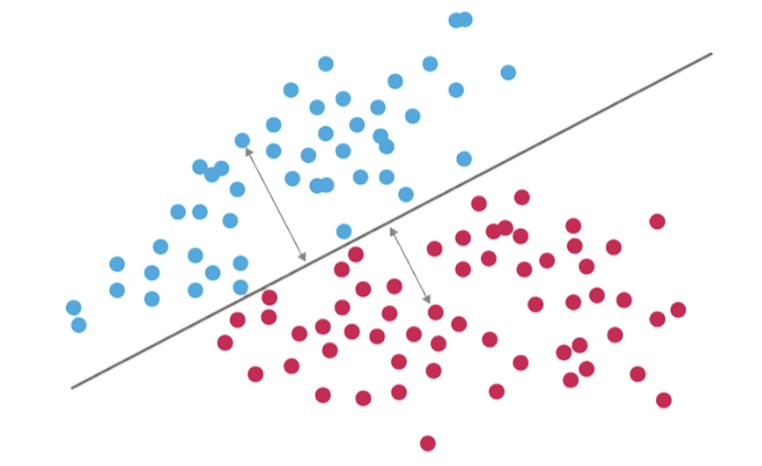
\includegraphics[width=.45\linewidth]{mi.png}
		\end{center}
\end{frame}


\begin{frame}{Пороговая функция потерь}
	
	\begin{wideitemize}
		\item  Разрывная функция
		\item  Можно использовать методы негладкой оптимизации, но это сложно
	\end{wideitemize}
	
	\[
	L(M_i) =[M_i < 0] = [y_i  \cdot  \langle w, x_i \rangle < 0]
	\]
	
	
	\begin{center}
		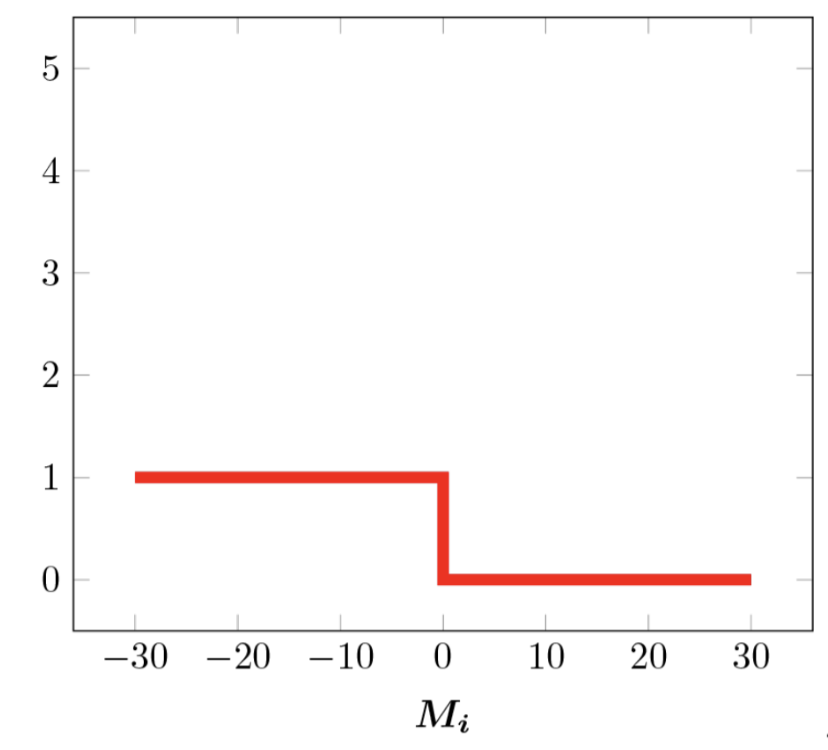
\includegraphics[width=.3\linewidth]{step.png}
	\end{center}
\end{frame}


\begin{frame}{Инженерный подход к классификации}

	\begin{wideitemize}
		\item  Возьмём любую гладкую оценку пороговой функции
		
		\[ [M < 0] \le \tilde{L}(M) \]
		
		\item  Оценим через неё функционал ошибки
		
		\[
		Q(a, X) \le \tilde{Q}(a, X) = \frac{1}{n} \sum_{i=1}^n \tilde L(M_i)
		\]
		
		\item Будем минимизировать получившуюся верхнюю оценку
	\end{wideitemize}
\end{frame}


\begin{frame}{Примеры оценок}
	\begin{wideitemize}
		\item  Логистическая (logloss): 
		
		\[
		\tilde L(M_i) = \ln(1 + \exp(-M_i))
		\]
		
		\item Экспоненциальная: 
		
		\[
		\tilde L(M_i) =  \exp(-M_i)
		\]
		
		\item Кусочно-линейная (если добавить $L_2$ регуляризатор, получим SVM): 
		
		\[
		\tilde L(M_i) =  \max(0, 1 - M_i)
		\]		
	\end{wideitemize}
\end{frame}


\begin{frame}{Примеры оценок}
	\begin{center}
		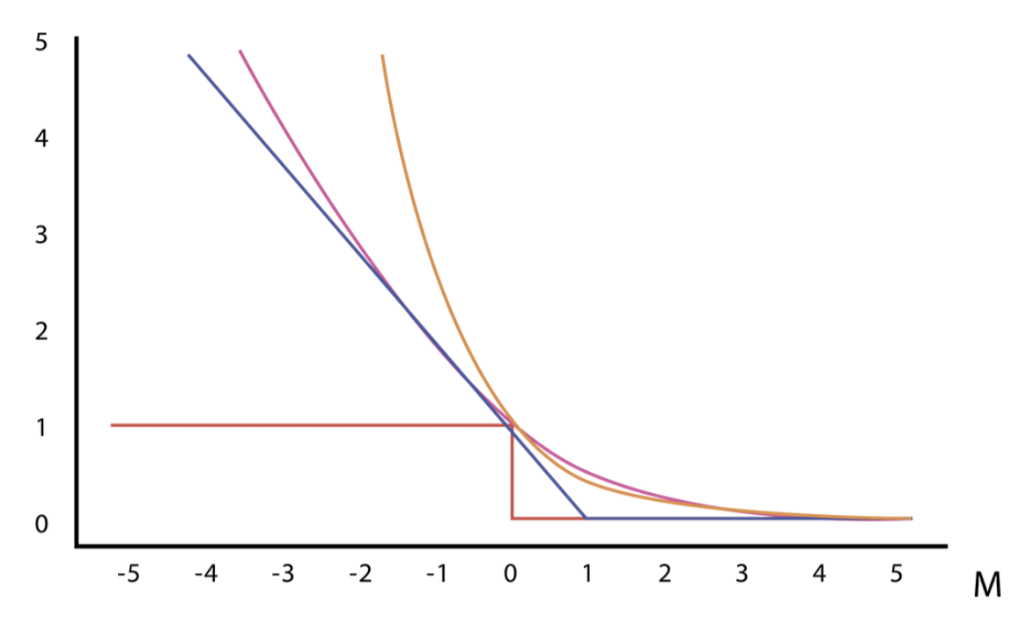
\includegraphics[width=.8\linewidth]{clfloss.png}
	\end{center}
\end{frame} 


\begin{frame}{Другой инженерный подход к logloss:}
	\begin{columns}[T] %
		\begin{column}{.49\textwidth}
				\begin{wideitemize}
						\item Пусть $y$ принимают значения $0$ и $1$ 
						\item Если $y = 1$, хотим большое $\hat p = \hat P(y = 1)$, но чем ближе $\hat p$ к $1$, тем меньше хотим его увеличить 
						\item Если $y = 0$, хотим большое $(1 - \hat p)$, получается функция потерь: 
						
						$$
						\logloss = - \frac{1}{n} \sum_{i=1}^n y_i \cdot \ln \hat p_i + (1 - y_i) \cdot \ln (1 - \hat p_i)
						$$
					\end{wideitemize}	
			\end{column}%
		\hfill%
		\begin{column}{.49\textwidth}
				\begin{center}
						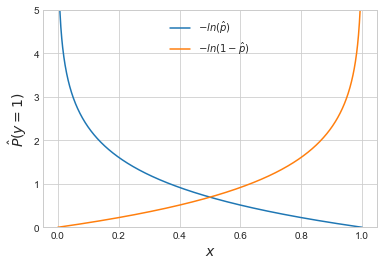
\includegraphics[width= 0.95\linewidth]{log_loss_05.png}
					\end{center}
			\end{column}%
	\end{columns}
\end{frame}
		
\begin{frame}{Вероятностный подход к logloss}
	\begin{equation*} 
			\begin{aligned}
					L(w) &=P(y_1, \ldots, y_n \mid X, w) =  \\ 
					&= P(y_1 \mid X,w) \cdot \ldots \cdot P(y_n \mid X, w) =  \\ 
					\mbox{ } \\  \pause 
					\ln L(w) & = \sum y_i \cdot \ln p_i + \sum(1 - y_i) \cdot \ln(1 - p_i) = \\ 
					&= \sum [ y_i \cdot \ln p_i + (1 - y_i) \cdot \ln(1 - p_i)] \to \max_{w} \\
					\mbox{ } \\  \pause 
					\logloss(w) & = -\ln L(w) = - \sum [ y_i \cdot \ln p_i + (1 - y_i) \cdot \ln(1 - p_i)]  \to \min_{w} 
				\end{aligned}
		\end{equation*}
\end{frame}


\begin{frame}{Резюме}
	\begin{wideitemize}
		\item Инженерный подход можно обобщить и для других метрик
		
		\item Например, есть гладка верхняя оценка для roc-auc и гладкий аналог f-меры
		
		\item На семинарах мы познакомимся с взвешенным logloss и focal-loss
	\end{wideitemize}
\end{frame}


\begin{transitionframe}
	\begin{center}
		\Huge Что такое регуляризация
	\end{center}
	% \centering \href{https://vk.com/skialz}{\includegraphics[scale = 0.25]{story.png}}
\end{transitionframe}


\begin{frame}{Регуляризация}
	\[
	Q(a, X) = \frac{1}{n}  \sum_{i=1}^n  \underbrace{L(y_i, a(x_i)) }_{\text{\textcolor{red}{Функция потерь}}} +  \lambda \cdot \underbrace{R(w)}_{\text{\textcolor{red}{Регуляризатор}}} \to  \min_w 
	\]
	
	\begin{wideitemize}
		\item \alert{Регуляризация}  — способ получить решение с определёнными свойствами
	\end{wideitemize}
\end{frame} 


\begin{frame}{Переобучение} 
	\begin{center}
		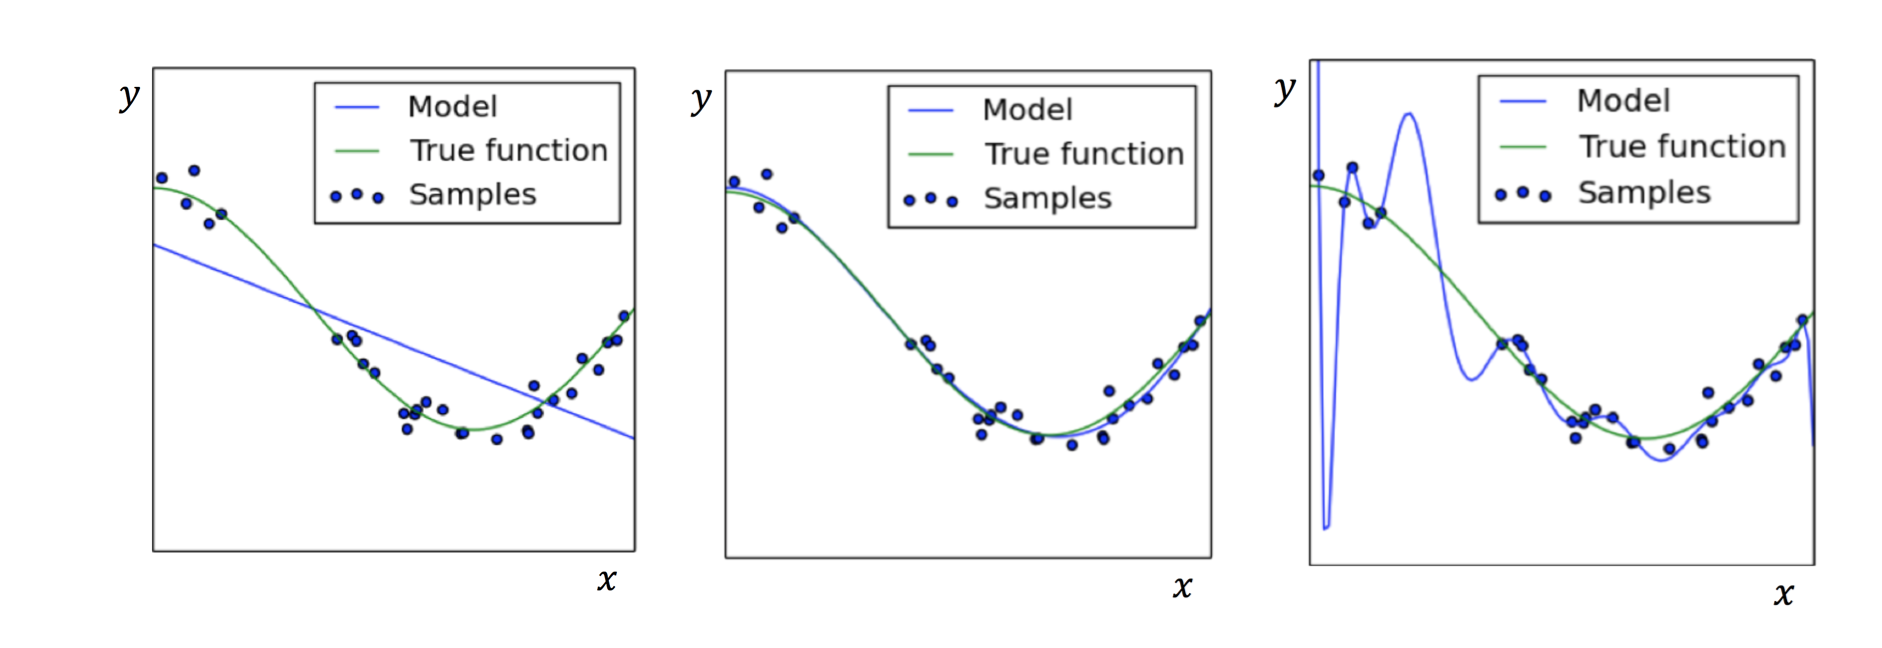
\includegraphics[scale=0.23]{overfit.png}
	\end{center}
\end{frame}


\begin{frame}{Переобучение это}
	\begin{wideitemize}
		
		\item  Модель запомнила данные, излишняя подгонка под обучающую выборку.
		
		\item  Модель слишком сложная, а данных слишком мало. и она в состоянии их запомнить.
		
		\item \alert{Признаки:}  высокое качество модели на обучающей выборке, низкое на тестовой, в случае линейных моделей высокие по модулю коэффициенты.
	\end{wideitemize}
\end{frame}


\begin{frame}{Чем навеяна регуляризация - сюжет 1}	
	\begin{wideitemize}
		\item В хорошей модели: $(0.634, 0.918, -0.626)$
		\item В переобученной модели: $(130.0, -525.8, \ldots, 102.6)$
		\item \alert{Мысль:} оштрафовать модель за излишне большие веса, это уберёт изгибы и сделает её проще

		\[
		Q(a, X) = \frac{1}{n}  \sum_{i=1}^n  \underbrace{L(y_i, a(x_i)) }_{\text{\textcolor{red}{Функция потерь}}} +  \lambda \cdot \underbrace{R(w)}_{\text{\textcolor{red}{Регуляризатор}}} \to  \min_w 
		\]
		
	\end{wideitemize}
\end{frame}


\begin{frame}{$L_2$ регуляризация (Ridge-регрессия)}
	
	\[L(\beta) + \lambda \cdot  \sum_{i=1}^d \beta_i^2  \to \min_{\beta}\]
	
	Задача оптимизации эквивалентна:
	
	\[
	\begin{cases} 
		L(w) \to \min_{w} \\
		\sum_{j=1}^d w_j^2 \le C \\
	\end{cases}
	\]
	
	\begin{center}
		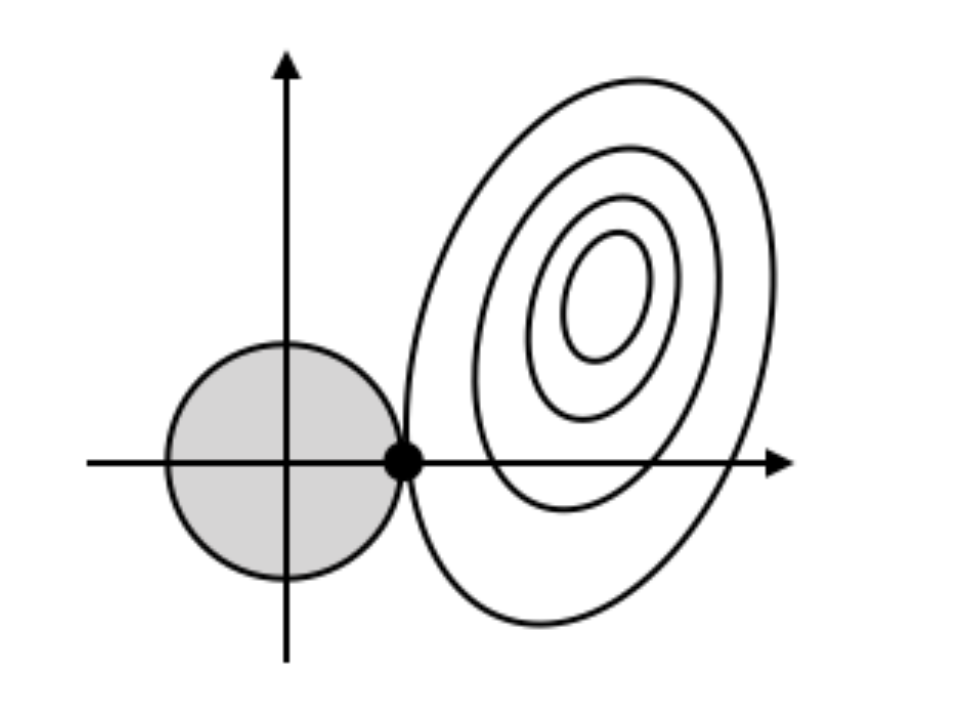
\includegraphics[width=0.33\paperwidth]{l2reg.png}
	\end{center}
\end{frame}


\begin{frame}{$L_1$ регуляризация (Lasso-регрессия)}
	
	\[L(w) + \lambda \cdot  \sum_{j=1}^d |w_j|  \to \min_{w}\]
	
	Задача оптимизации эквивалентна:
	
	\[
	\begin{cases} 
		L(w) \to \min_{w} \\
		\sum_{j=1}^d  |w_j| \le C \\
	\end{cases}
	\]
	
	\begin{center}
		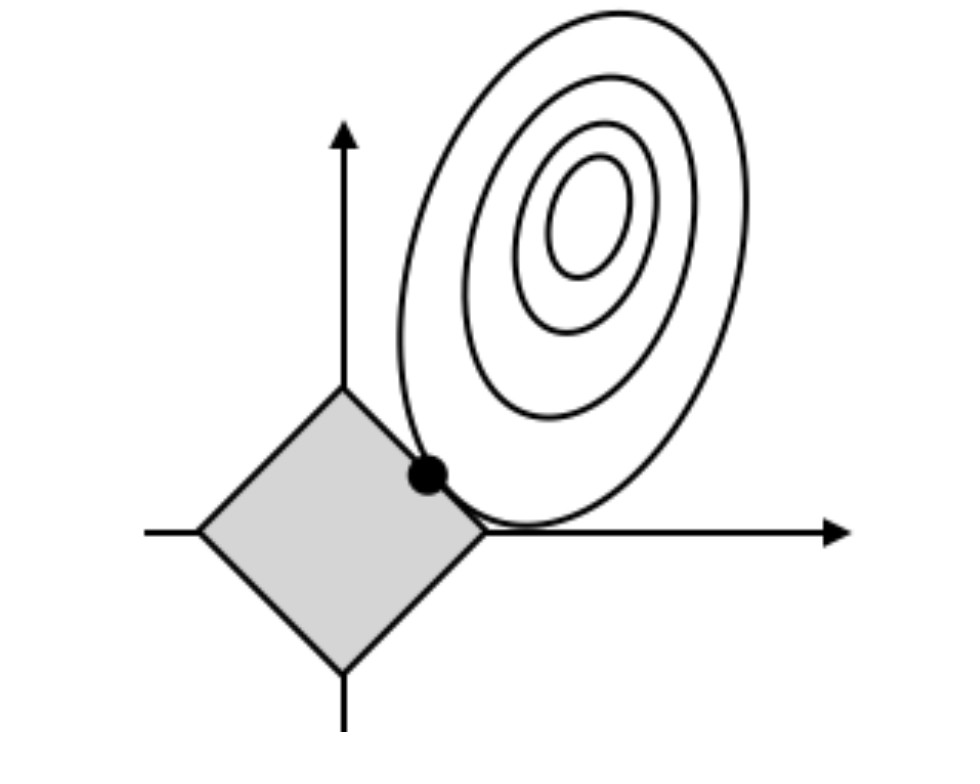
\includegraphics[width=0.3\paperwidth]{l1reg.png}
	\end{center}
\end{frame}


\begin{frame}{Коэффициент регуляризации}
	\begin{wideitemize}
		\item  Чем больше $\lambda$, тем ниже сложность модели и тем менее сложные закономерности она извлекает из данных;
		
		\item  Чем меньше $\lambda$, тем выше риск переобучения;
		
		\item  Нужен баланс $\Rightarrow$ подбор $\lambda$ по кросс-валидации.
		
	\end{wideitemize}
\end{frame}

\begin{frame}{Каверзные вопросы}
	\begin{wideitemize}
		\item  Вы заметили, что в регуляризатор не включается вес $w_0$? Почему? \pause 
		\item  Можно ли интерпретировать коэффициенты в Lasso или Ridge регрессии как изменение $y$ в среднем на $w_j$ единиц при росте $x_j$ на единицу? 
	\end{wideitemize}
\end{frame} 


\begin{frame}{$L_1$ vs $L_2$}
	\begin{wideitemize}
		\item $L_2$- регуляризатор: 
		\begin{enumerate}
			\item Штрафует модель за сложность
			\item Гладкий и выпуклый 
			\item Функция потерь дифференцируема, есть решение в явном виде
		\end{enumerate}
		
		\item $L_1$-регуляризатор:
		\begin{enumerate}
			\item Штрафует модель за сложность
			\item Негладкий
			\item Недифференцируемый, нет решения в явном виде
			\item Некоторые веса оказываются нулевыми, позволяет отбирать признаки
		\end{enumerate}
	\end{wideitemize}
\end{frame} 


\begin{frame}[plain]
	
	\begin{center}
		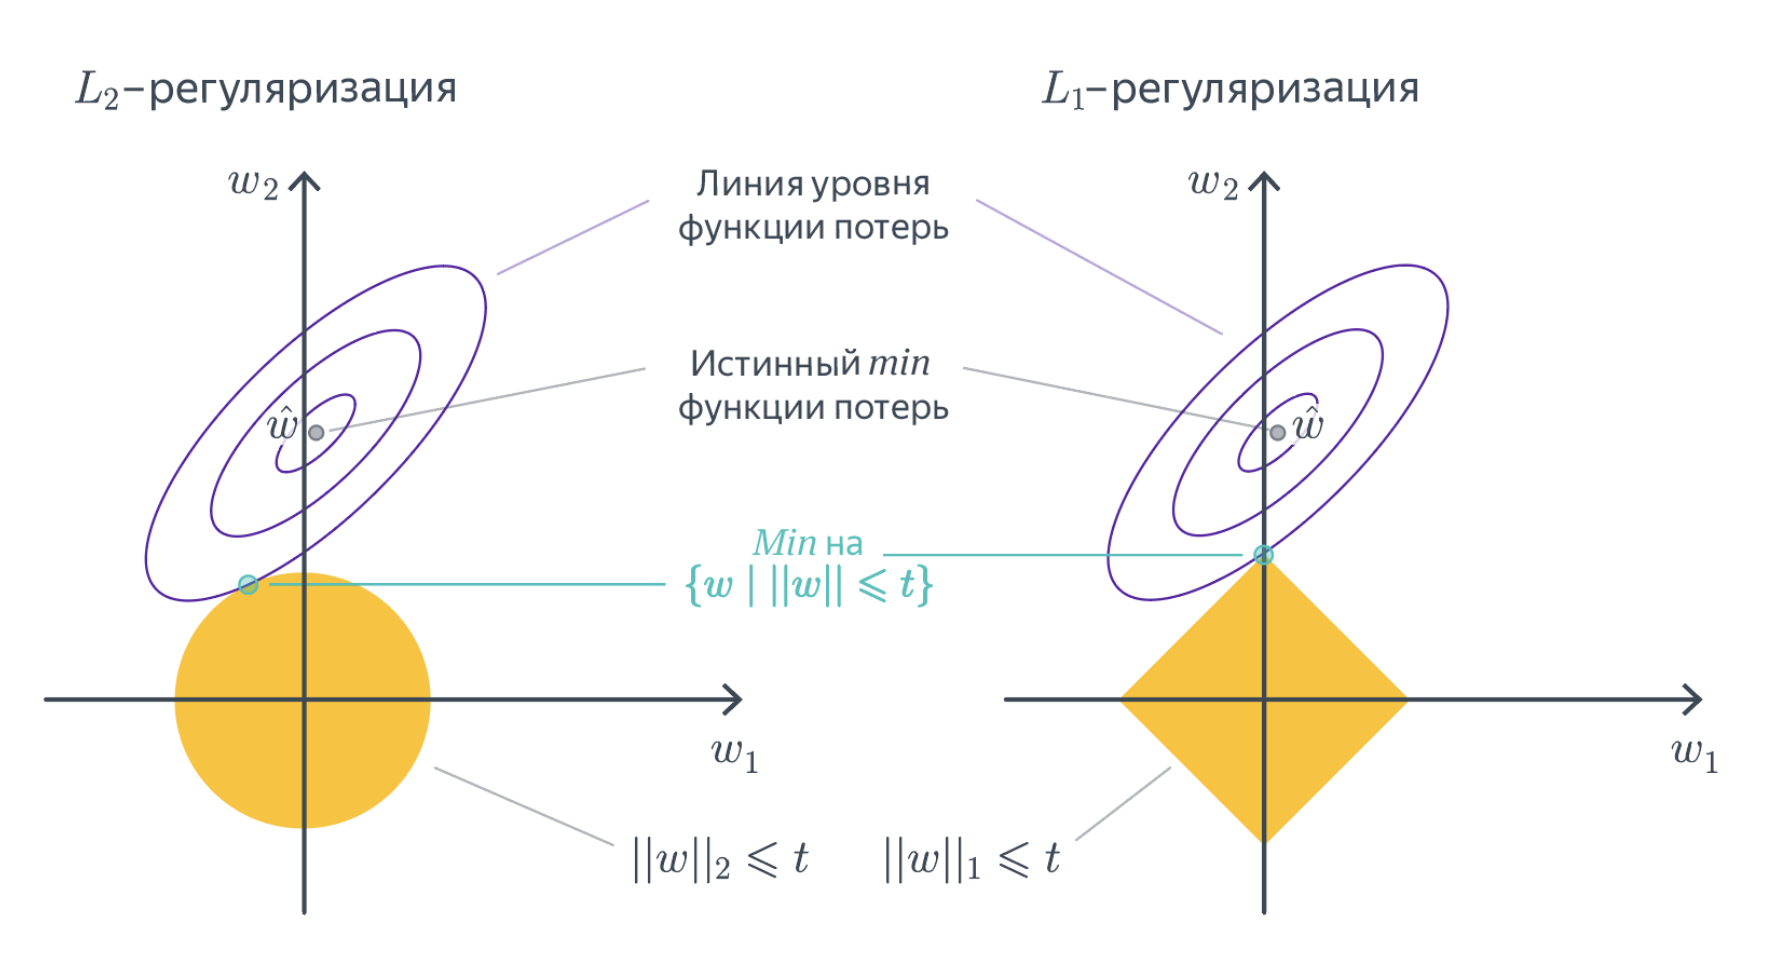
\includegraphics[width=0.87\paperwidth]{l1vsl2.png}
	\end{center}
\vfill
{\footnotesize
\color{blue}
\url{https://ml-handbook.ru/chapters/linear_models/intro}
}
\end{frame}


\begin{frame}{Мультиколлинеарность}
	\begin{wideitemize}
		
		\item \alert{Мультиколлинеарность  —} линейная зависимость признаков.
		
		\item Для любого $x_i$ из выборки существует набор $\alpha_1, \ldots, \alpha_d$ такой, что \[\alpha_1 x_{i1} + \ldots + \alpha_d x_{id} = \langle \alpha, x \rangle =  0.\]
		
	\end{wideitemize}
\end{frame} 


\begin{frame}{Мультиколлинеарность}
	\begin{wideitemize}
		\item Пусть мы нашли решение 
		
		\[ \hat w = \arg \min_{w} \frac{1}{n} \sum_{i=1}^n ( \langle w, x_i \rangle - y_i )^2 \]
		
		\item  Изменим вектор весов: $\tilde w = \hat w + t \cdot \alpha$
		
		\item Получаем, что 
		
		\[ \langle \tilde w, x \rangle =  \langle \hat w + t \cdot \alpha, x \rangle = \langle \hat w, x \rangle + t \cdot \langle \alpha, x \rangle = \langle \hat w, x \rangle  \]
		
		\item Бесконечно много оптимальных решений
	\end{wideitemize}
\end{frame} 


\begin{frame}{Мультиколлинеарность}
	\begin{wideitemize}
		\item Бесконечно много оптимальных решений
		
		\item Большая часть решений с огромными весами $\tilde w$ $\Rightarrow$ обладают плохой обобщающей способностью 
		
		\item  Регуляризация, накладывая штраф на коэффициенты, помогает выбрать среди бесконечного числа решений конкретное
	\end{wideitemize}
\end{frame} 


\begin{frame}{Регуляризация и байесовский подход}
	\begin{wideitemize}
		
		\item  На слайдах выше мы относились к регуляризации по-инженерному и ввели её для того, чтобы уменьшить абсолютное значение коэффициентов
		
		\item  Сущесвтует вероятностный взгляд на регуляризацию
		
		\item  С точки зрения байесовского подхода, регуляризация соотвествует заданию априорного распределения на коэффициенты
		
		\item Подробнее мы поговорим об этом на семинарах
	\end{wideitemize}
\end{frame}


\begin{transitionframe}
	\begin{center}
		\Huge  Разложение ошибки на смещение и разброс
	\end{center}
	% \centering \href{https://vk.com/skialz}{\includegraphics[scale = 0.25]{story.png}}
\end{transitionframe}
 
 
\begin{frame}{Разложение ошибки на смещение и разброс}
		\begin{wideitemize}
			
		\item Среднеквадратичную ошибку можно разложить на три составляющие:
	
				\[ MSE  = \sigma^2 +  Var( a(x) ) + bias(a(x))^2  \]
	
		\item $\sigma^2$  – неустранимая ошибка;
		
		\item $Var(a(x))$ – дисперсия прогноза, то насколько ошибка будет отличаться, если обучать модель на разных наборах данных;
		
		\item $bias^2(a(x))$ – средняя ошибка по всевозможным наборам данных;
		
		\item \alert{С первой ничего сделать не можем, на остальное можем влиять.}
		
		\item Мы докажем это разложение на следующих лекциях 
		
	\end{wideitemize}
\end{frame}


\begin{frame}{Разложение ошибки на смещение и разброс}
	\begin{center}
		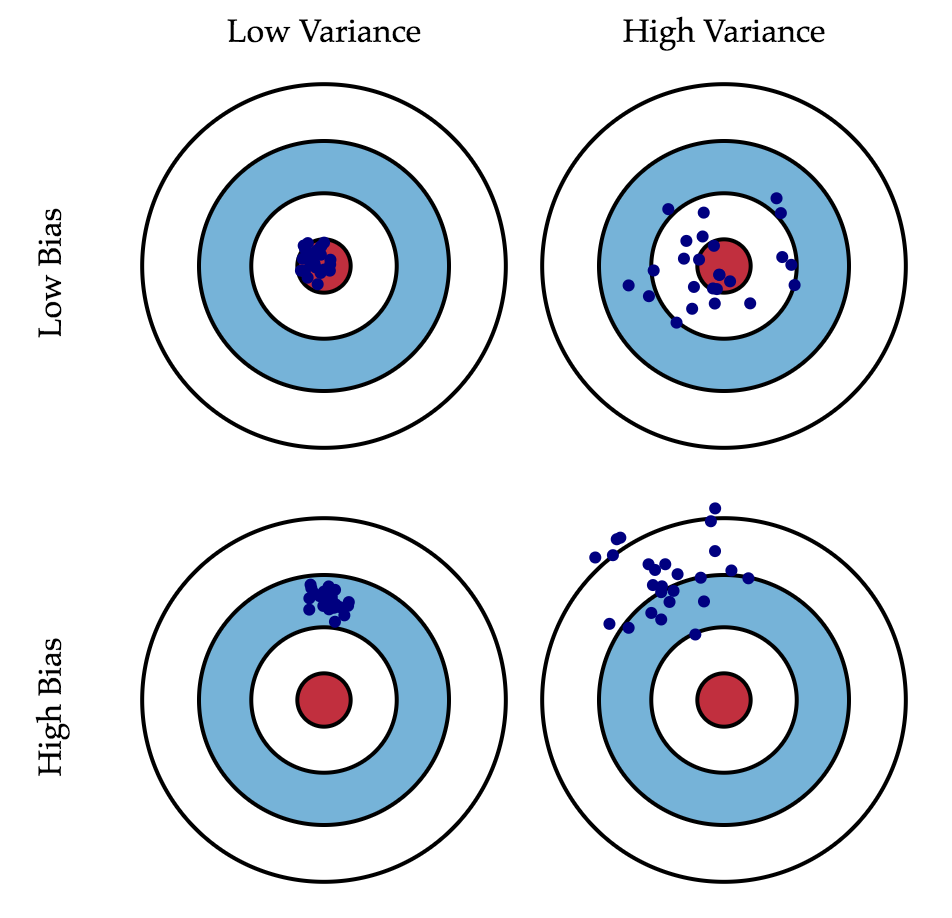
\includegraphics[scale=0.23]{est_var.png}
	\end{center}
\end{frame}


\begin{frame}{Разложение ошибки на смещение и разброс}
	\begin{wideitemize}
			
			\item  При увеличении сложности модели (рост числа оцениваемых параметров) смещение убывает, разброс растёт.
			
			\item Модель выучивает тренировочные данные и переобучается.  
			
			\item \alert{Иногда можно намеренно увеличивать смещение модели ради её стабильности.}
			
		\end{wideitemize}
\end{frame}


\begin{frame}{Разложение ошибки на смещение и разброс}
	\begin{center}
			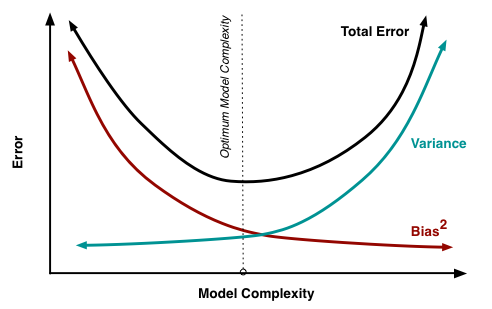
\includegraphics[scale=0.55]{est_var_2.png}
		\end{center}
\end{frame}


 \begin{frame}{Теорема Гаусса-Маркова}
	
	Предположим, что:
	
	\mbox{   }
	
	\begin{enumerate} 
		\item $y = X w + \varepsilon$;
		\item $X$ — детерминированная матрица размера $n \times k$ с полным столбцовым рангом;
		\item $E(\varepsilon) = 0, Var(\varepsilon) = \sigma^2 \cdot I_n$.
	\end{enumerate}
	
	\mbox{   }
	
	Тогда оценка метода наименьших квадратов \[\hat w = (X^TX)^{-1}X^Ty\] наиболее эффективная (в смысле наименьшей дисперсии) в классе линейных (по $y$) несмещённых оценок.
\end{frame}


\begin{frame}{Теорема Гаусса-Маркова и BVD}

	\begin{wideitemize}
		
		\item Среднеквадратичную ошибку можно разложить на три составляющие:
		
		\[ MSE  = \sigma^2 +  Var( a(x) ) + bias(a(x))^2  \]

		
		\item Теорема Гаусса-Маркова говорит, что $\hat y^{OLS}$ обладает нулевым смещением и наименьшим разбросом, то есть для любого другого несмещённого прогноза $\tilde y$ выполняется $Var(\tilde y) \ge Var( \hat y)$. 
		
		\item Прогноз можно сделать смещённым, но с меньшим разбросом с помощью регуляризации
	
	\end{wideitemize}
\end{frame}




\begin{frame}{Резюме по регуляризации}
	\begin{wideitemize}
		
		\item  \textcolor{blue}{Сюжет 1:} регуляризация помогает нащупать баланс между смещением и разбросом и получить  более точные прогнозы. 
		
		\item \textcolor{blue}{Сюжет 2:} если модель переобучилась, она сложная и извивается. Признак переобучения в линейной модели — большие веса. Регуляризатор вводит штраф за большие веса и даёт бой переобучению.
		
		\item \textcolor{blue}{Сюжет 3:} в случае мультиколлинеарности у нас бесконечно много решений. Многие с большими коэффициентами. Регуляризатор помогает выбрать решение \alert{с заданными свойствами:} маленькие коэффициенты. 
		
		\item В общем случае регуляризаторы помогают получать решения с желаемыми свойствами.
		
	\end{wideitemize}
\end{frame}


\end{document}
